%\documentclass[review]{cvpr}
\documentclass[final]{cvpr}

\usepackage{times}
\usepackage{epsfig}
\usepackage{graphicx}
\usepackage{amsmath}
\usepackage{amssymb}
%Path relative to the main .tex file 
\graphicspath{ {./images/} }
% Include other packages here, before hyperref.

% If you comment hyperref and then uncomment it, you should delete
% egpaper.aux before re-running latex.  (Or just hit 'q' on the first latex
% run, let it finish, and you should be clear).
\usepackage[pagebackref=true,breaklinks=true,colorlinks,bookmarks=false]{hyperref}


\def\cvprPaperID{****} % *** Enter the CVPR Paper ID here
\def\confYear{CVPR 2021}
%\setcounter{page}{4321} % For final version only


\begin{document}

%%%%%%%%% TITLE
\title{Survey On Machine Learning Paradigms For Phishing Website Detection}

\author{Madan Baduwal\textsuperscript{1}  \and Prakash Madai\textsuperscript{2} \and Tasnimul Alam \textsuperscript{3} \and Quan Yuan \textsuperscript{4} \\
\textsuperscript{\rmfamily\textbf{1}}Department of Computer Science, University of Texas Permian Basin\\
\texttt{\{baduwal\textunderscore m63609,madai\textunderscore p57558,alam\textunderscore m61291,yuan\textunderscore q\}@utpb.edu}}


\maketitle


%%%%%%%%% ABSTRACT
\begin{abstract}
   Phishing attacks continue to be a major security threat for individuals and organizations alike. 
   It causes billions of dollars in losses annually.
   Machine learning(ML) has shown great promise in detecting such attacks by identifying patterns and anomalies in large datasets.
   The tradeoff between feature selection and model selection is a tedious task in ML for phishing detection. 
   Low number of features are not enough for the generalizability of traditional machine learning algorithms i.e.For Logistic Regression(LR), Support Vector Machine(SVM), Random Forest(RF), XG boost and Naive Bayes(NB). 
   And it's tough for deep learning(DL) algorithms to learn features from ambiguities behaviour between phishing and non-phishing websites. 
   This paper presents a comprehensive survey of feature selection methods for various ML and ML paradigms that have been employed for the detection of phishing websites. 
   The survey also discusses various datasets, features, number of parameters in algorithms,training time-space complexity in phishing detection and compares the accuracies of different ML techniques.
   The results of this survey provide valuable insight into the current state of the art in phishing detection and can serve as a useful resource for researchers and practitioners working in this field.

\end{abstract}

%%%%%%%%% BODY TEXT
\section{Introduction}

Phishing websites have become a significant threat to online security. These websites are designed to trick users into revealing their sensitive information, such as passwords, credit card numbers, and other personal data. As the sophistication of phishing attacks increases, traditional anti-phishing techniques have become less effective. Machine learning has emerged as a promising approach to detect phishing websites in real-time.

Anti-Phishing Working Group(APWG) emphasizes that phishing attacks
have grown in recent years, Figures~\ref{fig:apwg-report} illustrates the total
number of phishing sites detected by APWG in the first quarter
of 2022 and the last quarter of 2021. During the third quarter of 2022, APWG recorded a staggering 1,270,883 phishing attacks, marking a new record and the most severe quarter for phishing observed by APWG to date. 
The total for August 2022 was 430,141 attacks,
which is the highest monthly total reported. 

\hspace*{-0.2in}
\begin{figure}[h]
   \centering
   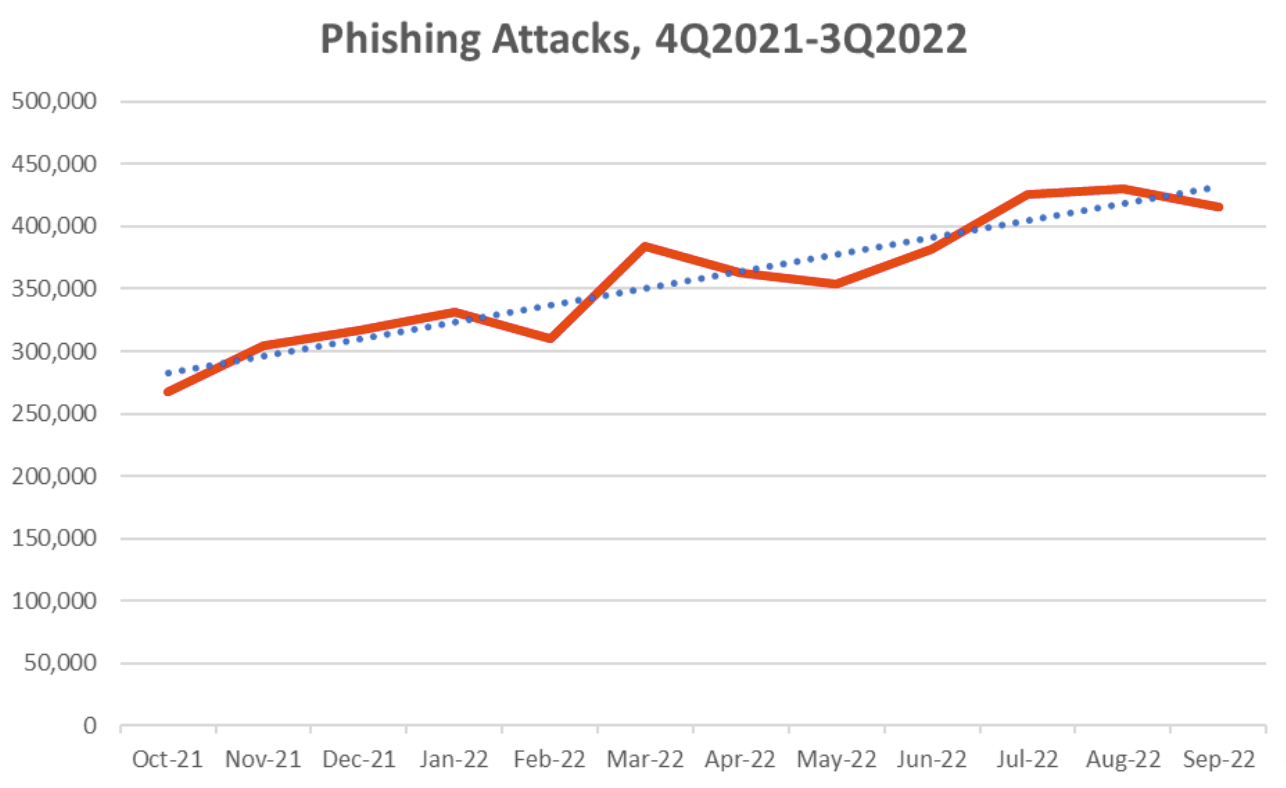
\includegraphics[width=8cm, height=5cm]{APWG-phishing-detection-report.png}
   \caption{Total number of phishing websites detected by APWG}
   \label{fig:apwg-report}
\end{figure}

The number of reported phishing attacks reported to APWG
has more than quintupled since the first quarter of 2020, when APWG observed 230,554 attacks.
The rise in Q3 2022 is attributable in part to increasing numbers of attacks reported against several
specific targets. These targets suffered from large numbers of attacks from persistent phishers.
Statistical Highlights for the 3rd Quarter 2022.



This paper presents a survey on machine learning paradigms for phishing website detection. The primary objective of this survey is to provide an overview of the state-of-the-art in machine learning-based anti-phishing techniques. The paper aims to review the existing literature on this topic, categorize the various machine learning paradigms used in phishing detection, and highlight their strengths and weaknesses.



The survey begins with a discussion of the fundamental concepts of phishing attacks, including their various types and characteristics. The paper then provides an overview of machine learning, including its various paradigms such as supervised learning, unsupervised learning, and reinforcement learning. The survey then proceeds to examine the existing research on machine learning-based phishing detection, categorizing the approaches based on the type of features used, the classification algorithm employed, and the evaluation metrics utilized.

Furthermore, the paper will provide a critical analysis of the current state-of-the-art, identifying the strengths and weaknesses of each machine learning paradigm in phishing detection. Finally, the survey will conclude by discussing the challenges and future research directions in machine learning-based anti-phishing techniques.

In conclusion, this paper's primary objective is to provide a comprehensive survey of machine learning paradigms for phishing website detection. The survey will be useful for researchers, practitioners, and policymakers in the field of cybersecurity, providing insights into the latest trends and developments in machine learning-based anti-phishing techniques.


\section{Background and Related Work}

\hspace*{-0.2in}
\begin{figure}[h]
   \centering
   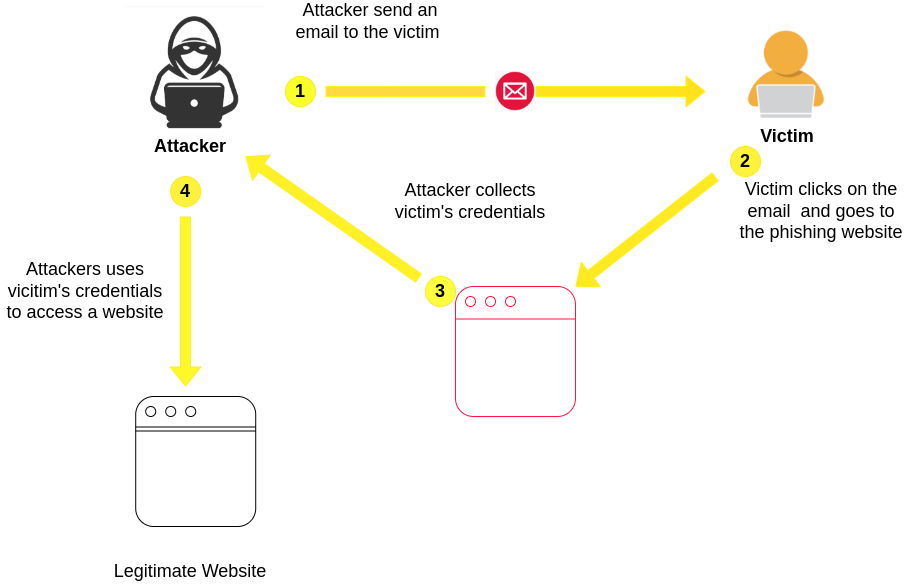
\includegraphics[width=8cm, height=5cm]{phishing-life-cycle.png}
   \caption{Phishing Life Cycle}
   % \label{fig:mesh1}
\end{figure}

\subsection{Phishing Techniques}
This section covers various phishing techniques that are commonly employed by criminals to trick individuals.

A.  Link manipulation

Phishing primarily revolves around links, with attackers utilizing various 
techniques to deceive users into clicking on them. 
One such technique involves manipulating the URL to 
mimic a legitimate one, such as representing 
malicious URLs as hyperlinks with legitimate names on websites. 
Another approach is to create misspelled URLs that closely resemble legitimate ones,
 for instance, facebuuk.com. However, there is a much more sophisticated variant of 
typosquatting known as IDN Spoofing, which involves the use of non-English characters that bear a 
striking resemblance to their English counterparts. For example, an attacker might use a Cyrillic "c" or "a" instead of the 
corresponding English letters, making it significantly more difficult to recognize the deception.

B. Filter evasion

Phishers often display the content of their fraudulent websites as images or use Adobe Flash to make it challenging for some phishing detection techniques to detect their malicious activities.
To counter this type of attack, optical character recognition (OCR) technology must be employed.

C. Website forgery

In this form of attack, phishers manipulate the JavaScript code of a legitimate website to carry out phishing activities. 
These types of attacks, also referred to as cross-site scripting, are exceptionally difficult to detect since the victim is interacting with a genuine website.

D. Covert redirect

This attack is aimed at websites that use the OAuth 2.0 and OpenID protocols. 
In this scenario, when attempting to grant token access to a legitimate website, users inadvertently provide their token to a malicious service. 
Nevertheless, this technique has received little attention due to its limited significance.

E. Social engineering

Social engineering phishing is a deceptive attack that employs psychological manipulation to trick users into divulging their security information. 
This type of attack typically involves multiple steps: first, the phisher researches the potential vulnerabilities of their targets. 
Next, the phisher attempts to gain the target's trust before finally creating a situation where the target unwittingly discloses important information. 
Social engineering phishing techniques include baiting, scareware, pretexting, and spear phishing.
\section{Datasets And Approaches}

\subsection{Dataset Descriptions}

Data are the source of each approach and proves to be a vital influence for the per-formance. There are two methods to collect data: loading published datasets and pulling
URLs directly from the Internet. Table 1 shows several major data sources. In these three
published datasets, every row’s data object contains several features extracted from a URL
and a label of classes. The original URL strings could be collected from websites by running
open API or data mining scripts.

\begin{figure*}
   \begin{center}
      Table 1. Major data sources for detecting phishing websites.
      \begin{tabular}{ccc}
         \hline
         Data Source & Type & Remarks \\
         \hline
         UCI [22] & Published dataset & $\begin{array}{c}1,055 \text { instances with } \\ 30 \text { features }\end{array}$ \\
         \hline
         Mendeley [23] & Published dataset & $\begin{array}{c}10,000 \text { instances with } \\ 48 \text { features }\end{array}$ \\
         \hline
         ISCX-URL-2016 [25] & Published dataset & $\begin{array}{c}35,000 \text { legitimate URLs } \\ \text { 10,000 phishing URLs }\end{array}$ \\
         \hline
         $\begin{array}{c}\text { https: / phishtank.com } \\ \text { (accessed on 18 July 2021) [18] }\end{array}$ & Walid phishing URLs &  \\
         \hline
         $\begin{array}{c}\text { https: / openphish.com } \\ \text { (accessed on 18 July 2021) }\end{array}$ & Valid phishing URLs &  \\
         \hline
         $\begin{array}{c}\text { https: / commoncrawl.org / } \\ \text { (accessed on 18 July 2021) }\end{array}$ & Wegite & Legitimate URLs \\
         \hline
         $\begin{array}{c}\text { https: / www.alexa.com / } \\ \text { (accessed on 18 July 2021) [20] }\end{array}$ & Website & Webte URLs \\
         \hline
         \end{tabular}
   \end{center}
      % \caption{Example of a short caption, which should be centered.}
   \label{fig:short}
   \end{figure*}

\subsection{Feature Engineering}

Feature selection is the process of automatically selecting important features which
contribute the most to the machine learning model. Having closely relevant features in
the input can enhance the performance of the model, decrease training time (especially in
deep learning models), and reduce overfitting issues. Generally, feature selection method-
ologies could be classified into three categories: the filter method, wrapper method, and
embedded method.

\subsection{Detection Approaches}

\hspace*{-0.9in}
\begin{figure}[h]
   \centering
   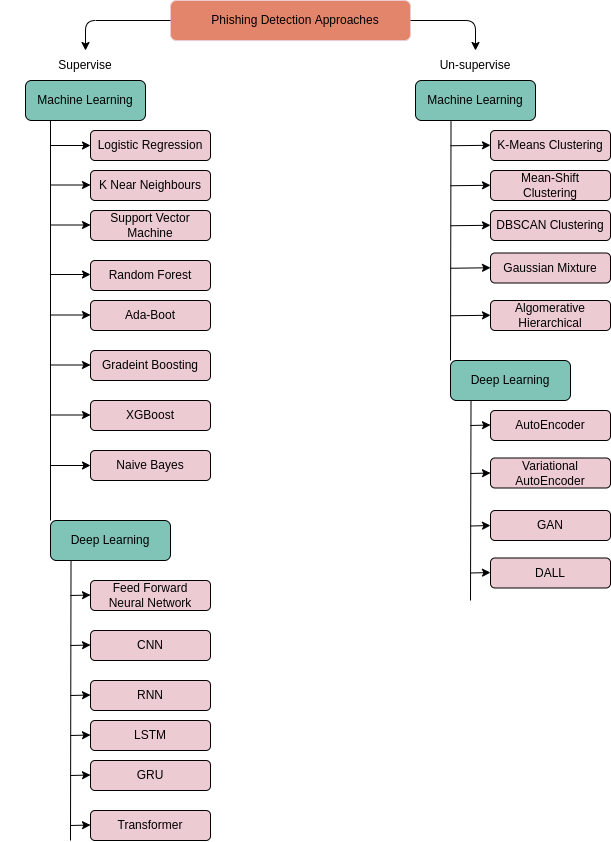
\includegraphics[width=8.5cm, height=14cm]{phishing-detection-approaches.png}
   \caption{Phishing Detection Approaches}
   % \label{fig:mesh1}
\end{figure}

1. Logistic regression(image+equation)


Logistic Regression is a classification algorithm used to
assign observations to a discrete set of classes. Unlike linear
regression which outputs continuous number values, Logistic
Regression transforms its output using the logistic sigmoid
function to return a probability value which can then be
mapped to two or more discrete classes. Logistic regression
works well when the relationship in the data is almost linear
despite if there are complex nonlinear relationships between
variables, it has poor performance. Besides, it requires more
statistical assumptions before using other techniques.

2. K Near Neighbors

K-Nearest Neighbors (KNN) is one of the simplest algo-
rithms used in machine learning for regression and classifi-
cation problems which is non-parametric and lazy. In KNN
there is no need for an assumption for the underlying data
distribution. KNN algorithm uses feature similarity to predict
the values of new datapoints which means that the new data
point will be assigned a value based on how closely it matches
the points in the training set. The similarity between records
can be measured in many different ways. Once the neighbors
are discovered, the summary prediction can be made by
returning the most common outcome or taking the average.
As such, KNN can be used for classification or regression
problems. There is no model to speak of other than holding
the entire training dataset.


3. Support Vector Machine

Support vector machines (SVMs) are one of the most popu-
lar classifiers. The idea behind SVM is to get the closest point
between two classes by using the maximum distance between
classes. This technique is a supervised learning model used
for linear and nonlinear classification. Nonlinear classification
is performed using a kernel function to map the input to a
higher-dimensional feature space. Although SVMs are very
powerful and are commonly used in classification, it has some
weakness. They need high calculations to train data. Also, they
are sensitive to noisy data and are therefore prone to over-
fitting. The four common kernel functions at the SVM are
linear, RBF (radial basis function), sigmoid, and polynomial,
which is listed in Table I. Each kernel function has particular
parameters that must be optimized to obtain the best result.

4.  Random Forest

Random forest is a popular machine learning algorithm that is widely used in data science and research. 
It is an ensemble learning method that combines multiple decision trees to create a robust and accurate model. 
In random forest, each decision tree is constructed using a subset of the available features and training data, and the final prediction is made by aggregating the results of all the trees. 
This approach helps to reduce overfitting and improve the overall performance of the model. 
Random forest can be applied to a wide range of research problems, including classification, regression, and feature selection, making it a versatile and powerful tool in data analysis.

Mahmoud Othman 

4. Ada-Boost

From some aspects, Ada-boost is like Random Forest, the
Ada-Boost classification like Random Forest groups weak
classification models to form a strong classifier. A single
model may poorly categorize objects. But if we combine
several classifiers by selecting a set of samples in each iteration
and assign enough weight to the final vote, it can be good
for the overall classification. Trees are created sequentially
as weak learners and correcting incorrectly predicted samples
by assigning a larger weight to them after each round of
prediction. The model is learning from previous errors. The
final prediction is the weighted majority vote (or weighted
median in case of regression problems). In short Ada-Boost
algorithm is repeated by selecting the training set based on the
accuracy of the previous training. The weight of each classifier
trained in each iteration depends on the accuracy obtained
from previous ones [19].

5. Gradeint Boosting

Gradient Boosting trains many models incrementally and
sequentially. The main difference between Ada-Boost and
Gradient Boosting Algorithm is how algorithms identify the
shortcomings of weak learners like decision trees. While the
Ada-Boost model identifies the shortcomings by using high
weight data points, Gradient Boosting performs the same
methods by using gradients in the loss function. The loss func-
tion is a measure indicating how good the models coefficients
are at fitting the underlying data. A logical understanding of
loss function would depend on what we are trying to optimize.
[20]

6. GBoost

XGBoost is a refined and customized version of a Gradient
Boosting to provide better performance and speed. The most
important factor behind the success of XGBoost is its scala-
bility in all scenarios. The XGBoost runs more than ten times
faster than popular solutions on a single machine and scales
to billions of examples in distributed or memory-limited set-
tings. The scalability of XGBoost is due to several important
algorithmic optimizations. These innovations include a novel
tree learning algorithm for handling sparse data; a theoretically
justified weighted quantile sketch procedure enables handling
instance weights in approximate tree learning. Parallel and dis-
tributed computing make learning faster which enables quicker
model exploration. More importantly, XGBoost exploits out-
of-core computation and enables data scientists to process
hundreds of millions of examples on a desktop. Finally, it
is even more exciting to combine these techniques to make
an end-to-end system that scales to even larger data with the
least amount of cluster resources.

7. Artificial Neural Networks

Artificial neural networks (ANNS) are a learning model
roughly inspired by biological neural networks. These models
are multilayered, each layer containing several processing
units called neurons. Each neuron receives its input from
its adjacent layers and computes its output with the help
of its weight and a non-linear function called the activation
function. In feed-forward neural networks like in 3, data flows
from the first layer to the last layer. Different layers may
perform different transformations on their input. The weights
of neurons are set randomly at the start of the training and
they are gradually adjusted by the help of the gradient descent
method to get close to the optimal solution. The power of
neural networks is due to the non-linearity of hidden nodes.
As a result, introducing non-linearity in the network is very
important so that you can learn complex functions [22]
\section{Results and discussion}

\subsection{Evaluation Matrices}

\subsection{Experimental Results}

% \pagebreak 
% Table 1. Major data sources for detecting phishing websites.
% \begin{center}
%    \begin{tabular}{ccc}
%    \hline
%    Classifier & recall & precision  \\
%    \hline
%    UCI [22] & Published dataset & $\begin{array}{c}1,055 \text { instances with } \\ 30 \text { features }\end{array}$ \\
%    \hline
%    Mendeley [23] & Published dataset & $\begin{array}{c}10,000 \text { instances with } \\ 48 \text { features }\end{array}$ \\
%    \hline
%    ISCX-URL-2016 [25] & Published dataset & $\begin{array}{c}35,000 \text { legitimate URLs } \\ \text { 10,000 phishing URLs }\end{array}$ \\
%    \hline
%    $\begin{array}{c}\text { https: / phishtank.com } \\ \text { (accessed on 18 July 2021) [18] }\end{array}$ & Walid phishing URLs &  \\
%    \hline
%    $\begin{array}{c}\text { https: / openphish.com } \\ \text { (accessed on 18 July 2021) }\end{array}$ & Valid phishing URLs &  \\
%    \hline
%    $\begin{array}{c}\text { https: / commoncrawl.org / } \\ \text { (accessed on 18 July 2021) }\end{array}$ & Wegite & Legitimate URLs \\
%    \hline
%    $\begin{array}{c}\text { https: / www.alexa.com / } \\ \text { (accessed on 18 July 2021) [20] }\end{array}$ & Website & Webte URLs \\
%    \hline
%    \end{tabular}
%    \end{center}

{\small
\bibliographystyle{ieee_fullname}
\bibliography{egbib}
\nocite{*}
}

\end{document}
